\chapter{Methodology}
Methodology in research refers to the systematic approach or framework used by researchers to conduct their study, gather data, analyze findings, and draw conclusions.
It encompasses the strategies, techniques, procedures, and tools employed to address research questions, test hypotheses, or achieve research objectives.
Methodology serves as a roadmap that guides the entire research process, ensuring rigor, reliability, and validity in the investigation.

Key components of methodology in research include the following.

\subsection{Research Design}
The overall plan or structure of the study, including its purpose, scope, and objectives.
This may involve choosing between experimental, observational, qualitative, quantitative, or mixed methods research designs.
    
\subsection{Data Collection Methods}
The specific techniques and procedures used to gather relevant data or information for analysis.
This could include surveys, interviews, experiments, observations, archival research, or data mining.
    
\subsection{Sampling Strategy}
The process of selecting a representative subset of individuals, cases, or data points from a larger population for study.
This involves decisions about sample size, sampling techniques, and sampling frame.
    
\subsection{Data Analysis Techniques}
The methods used to analyze and interpret the collected data.
This may include statistical analysis, qualitative coding, content analysis, thematic analysis, or other analytical approaches.
    
\subsection{Validity and Reliability Considerations} 
Measures taken to ensure the validity and reliability of the research findings.
This includes strategies to minimize bias, control for confounding variables, establish internal and external validity, and assess the consistency and repeatability of results.
    
\subsection{Ethical Considerations}
Adherence to ethical principles and guidelines in conducting research, particularly concerning the protection of human subjects, confidentiality, informed consent, and avoiding conflicts of interest.
    
\subsection{Timeline and Resources}
Planning and scheduling the research activities, allocating resources (such as funding, personnel, and equipment), and establishing milestones and deadlines for completion.
    
\subsection{Theoretical Framework}
The underlying theoretical perspectives, concepts, or models that inform the research design and guide data collection, analysis, and interpretation.
    
\subsection{Limitations and Delimitations}
Acknowledgment of the constraints, limitations, and boundaries of the study, including factors that may impact the generalizability or applicability of the findings.
    
\subsection{Iterative Process}
Recognizing that research methodology is often iterative, with researchers refining their approach based on preliminary findings, feedback, and emerging insights.


Overall, methodology in research provides a systematic and structured framework for conducting rigorous and valid investigations, ensuring that research findings are credible, trustworthy, and meaningful.


\section{Common Methodologies in Mathematics Research}
In mathematics research, several methodologies are commonly used to investigate problems, develop theories, and prove conjectures.
Some of the most common methodologies include the following.

\subsection{Analytical Methods}
Analytical methods involve rigorous reasoning and logical deduction to study mathematical objects and phenomena.
This often includes developing mathematical models, formulating conjectures, and proving theorems using deductive reasoning and formal logic.

\subsection{Computational Methods}
Computational methods involve using computers to perform numerical simulations, calculations, and experiments.
This approach is particularly useful for solving complex mathematical problems, generating data, and exploring mathematical structures that are difficult to analyze analytically.

\subsection{Experimental Methods}
Experimental methods involve conducting experiments or observations to gather empirical data and test hypotheses in mathematics.
While less common in pure mathematics, experimental mathematics is often used in applied and computational mathematics to validate conjectures, explore patterns, and discover new phenomena.

\subsection{Algorithmic Methods}
Algorithmic methods involve designing and analyzing algorithms to solve mathematical problems efficiently.
This includes developing algorithms for numerical computation, optimization, graph theory, cryptography, and other areas of mathematics.

\subsection{Statistical Methods}
Statistical methods involve analyzing data and making inferences using statistical techniques such as regression analysis, hypothesis testing, and Bayesian inference.
This approach is commonly used in mathematical statistics, probability theory, and data analysis.

\subsection{Geometric Methods}
Geometric methods involve studying mathematical objects and structures using geometric techniques and visualizations.
This includes methods from differential geometry, algebraic geometry, topology, and geometric group theory.

\subsection{Topological Methods}
Topological methods involve studying properties of spaces and mappings that are preserved under continuous deformations, such as homeomorphisms and homotopies.
This approach is commonly used in algebraic topology, differential topology, and geometric topology.

\subsection{Combinatorial Methods}
Combinatorial methods involve studying discrete structures and counting techniques to solve problems in mathematics.
This includes combinatorial enumeration, graph theory, combinatorial optimization, and discrete mathematics.

\subsection{Modeling and Simulation}
Modeling and simulation involve constructing mathematical models to describe real-world phenomena and simulating their behavior using mathematical tools and techniques.
This approach is commonly used in mathematical modeling, applied mathematics, and mathematical physics.

\subsection{Interdisciplinary Approaches}
Many mathematical research projects involve interdisciplinary collaboration with researchers from other fields, such as physics, biology, engineering, economics, and computer science.
These projects often require combining mathematical methods with domain-specific knowledge and techniques to address complex problems.

These methodologies are not mutually exclusive, and researchers often combine multiple approaches to tackle mathematical problems from different angles. The choice of methodology depends on the nature of the problem, the available resources, and the researcher's expertise and preferences.



\section{Graphical Models}
\LaTeX has a lot of nice functionality for creating various types of
plots and diagrams.
Check out the nice graphs in Figure \ref{tikz:graphs}.

\begin{figure}[ht]
  \centering
  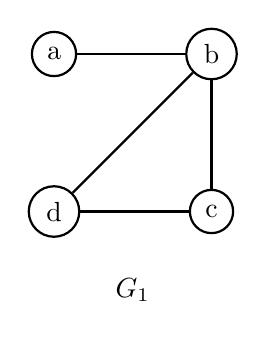
\begin{tikzpicture}
    \begin{scope}[every node/.style={circle,thick,draw}]
      \node (a) at (0,2) {a};
      \node (b) at (2,2) {b};
      \node (c) at (2,0) {c};
      \node (d) at (0,0) {d};
    \end{scope}
    \begin{scope}[every edge/.style={draw=black,thick}]
      \path (a) edge (b);
      \path (b) edge (c);
      \path (b) edge (d);
      \path (c) edge (d);
    \end{scope}
    \node () at (1,-1) {$G_1$};
  \end{tikzpicture}
  \hspace{1.5cm}
  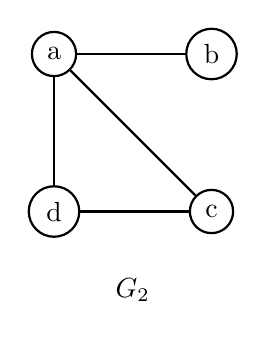
\begin{tikzpicture}
    \begin{scope}[every node/.style={circle,thick,draw}]
      \node (1) at (0,2) {a};
      \node (2) at (2,2) {b};
      \node (3) at (2,0) {c};
      \node (4) at (0,0) {d};
    \end{scope}
    \begin{scope}[every edge/.style={draw=black,thick}]
      \path (1) edge (2);
      \path (1) edge (3);
      \path (1) edge (4);
      \path (3) edge (4);
    \end{scope}
    \node () at (1,-1) {$G_2$};
  \end{tikzpicture}
  \caption{Nice pictures}
  \label{tikz:graphs}
\end{figure}

\section{Vector Spaces}

A \textbf{vector space} $V$ over a field $\mathbb{F}$ is a set equipped with two operations:

\begin{itemize}
    \item Vector addition: $+: V \times V \rightarrow V$, denoted as $(\mathbf{v}, \mathbf{w}) \mapsto \mathbf{v} + \mathbf{w}$.
    \item Scalar multiplication: $\cdot: \mathbb{F} \times V \rightarrow V$, denoted as $(\lambda, \mathbf{v}) \mapsto \lambda \mathbf{v}$.
\end{itemize}
These operations must satisfy the following properties for all $\mathbf{u}, \mathbf{v}, \mathbf{w} \in V$ and $\lambda, \mu \in \mathbb{F}$:

\begin{enumerate}
    \item \textbf{Addition is commutative}: $\mathbf{u} + \mathbf{v} = \mathbf{v} + \mathbf{u}$.
    \item \textbf{Addition is associative}: $(\mathbf{u} + \mathbf{v}) + \mathbf{w} = \mathbf{u} + (\mathbf{v} + \mathbf{w})$.
    \item \textbf{Additive identity}: There exists a vector $\mathbf{0} \in V$ such that $\mathbf{v} + \mathbf{0} = \mathbf{v}$ for all $\mathbf{v} \in V$.
    \item \textbf{Additive inverse}: For every vector $\mathbf{v} \in V$, there exists a vector $-\mathbf{v} \in V$ such that $\mathbf{v} + (-\mathbf{v}) = \mathbf{0}$.
    \item \textbf{Scalar multiplication is distributive over vector addition}: $\lambda (\mathbf{v} + \mathbf{w}) = \lambda \mathbf{v} + \lambda \mathbf{w}$.
    \item \textbf{Scalar multiplication is distributive over scalar addition}: $(\lambda + \mu) \mathbf{v} = \lambda \mathbf{v} + \mu \mathbf{v}$.
    \item \textbf{Scalar multiplication is associative}: $(\lambda \mu) \mathbf{v} = \lambda (\mu \mathbf{v})$.
    \item \textbf{Scalar multiplication identity}: $1 \cdot \mathbf{v} = \mathbf{v}$, where $1$ is the multiplicative identity in $\mathbb{F}$.
\end{enumerate}


\section{Dirac Notation}
Dirac notation, also known as bra-ket notation, is a powerful and concise mathematical notation used extensively in quantum mechanics.
It was introduced by the physicist Paul Dirac and provides a convenient way to represent vectors, linear operators, and inner products in quantum mechanics.
Here's a breakdown of the components of Dirac notation:

\begin{description}
  \item[Ket notation $\ket{\psi}$:]
  A ket is represented by a column vector enclosed within vertical bars.
  It represents a state vector in a complex vector space.
  For example, $\ket{\psi}$ could represent the state of a quantum system.

  \item[Bra notation $\bra{\psi}$:]
  A bra is represented by a row vector enclosed within angular brackets.
  It represents the complex conjugate transpose of a ket vector.
  If $\ket{\psi}$ represents a state vector, then $\ket{\psi}$ represents the corresponding bra vector.

  \item[Inner product ($\braket{\psi \mid \psi}$):]
  The inner product of two vectors is represented by placing a bra vector on the left and a ket vector on the right, enclosed within angular brackets.
  It yields a complex number and is a measure of the "overlap" between the two vectors.
  In quantum mechanics, the inner product is used to calculate probabilities and to determine the expectation values of observables.

  \item[Outer product ($\ket{\psi}\bra{\phi}$):]
  The outer product of two vectors is represented by placing a ket vector on the left and a bra vector on the right.
  It results in a linear operator known as a ket-bra or dyad, which maps one vector to another.
  In quantum mechanics, outer products are used to represent quantum operators.

  \item[Operators ($A\ket{\psi}$):]
  If $A$ is a linear operator, its action on a ket vector $\ket{\psi}$ is represented by placing the operator to the left of the ket vector.
  This notation shows the result of applying the operator to the state vector.
\end{description}
Dirac notation offers several advantages:
\begin{description}
    \item[Clarity and Conciseness:]
    It provides a concise representation of complex mathematical objects, making expressions and calculations easier to write and understand.
    \item[Flexibility:]
    It can be easily extended to represent complex operations and concepts in quantum mechanics, such as composite systems, entanglement, and measurement.
    \item[Computational Efficiency:]
    Dirac notation simplifies many calculations in quantum mechanics, such as computing inner products, expectation values, and transition probabilities.
\end{description}
Overall, Dirac notation is a fundamental tool in quantum mechanics, enabling physicists to express and manipulate quantum states and operations in a clear and efficient manner.
